\documentclass[12pt, a4paper]{report}

% Packages for fonts, math, and layout
\usepackage{mathptmx} % Using a safer alternative for Times font
\usepackage{amsmath}
\usepackage{amssymb}
\usepackage{geometry}
\geometry{a4paper, margin=1in}
\usepackage{setspace}
\onehalfspacing

% Packages for Images and Grids 
\usepackage{graphicx}
\usepackage{subcaption} 
\usepackage[framemethod=tikz]{mdframed} % For nice boxes

% Code formatting
\usepackage{listings}
\usepackage{xcolor}
\lstset{
    language=Python,
    basicstyle=\ttfamily\small,
    keywordstyle=\color{blue}\bfseries,
    stringstyle=\color{red},
    commentstyle=\color{green!60!black},
    numbers=left,
    numberstyle=\tiny\color{gray},
    stepnumber=1,
    breaklines=true,
    frame=single,
    captionpos=b,
    showstringspaces=false
}

% Hyperlinks
\usepackage{hyperref}
\hypersetup{colorlinks=true, linkcolor=blue, urlcolor=cyan, citecolor=blue}

\title{\Huge \textbf{A Python-Based Approach to Animate Geometry and Data}}
\author{
    \Large \textbf{Shubham Tiwari} \\[1ex]
    \normalsize \textit{Supervisor:} \textbf{Dr. J. V. Ramani} \\
    \normalsize \textit{Co-Supervisor:} \textbf{Ms. Ishver Rani Manchanda}
}
\date{}

\begin{document}

\maketitle

\begin{abstract}
Mathematical concepts are traditionally communicated through symbolic expressions and static diagrams. While such representations are mathematically precise, they often fail to illustrate the dynamic nature of geometric transformations and functional behavior. This work proposes a Python-based computational approach for animating mathematical structures, with the aim of improving conceptual understanding through visual and dynamic representations of mathematical motion. 

This chapter primarily focuses on two-dimensional geometric and analytical visualizations. Using Python libraries such as NumPy and Matplotlib, several classical mathematical problems are animated, including loci of points, equivalent norms, and the classical sliding ladder problem from coordinate geometry. In these examples, implicit equations are converted into parametric laws, allowing us to simulate spatial motion and transformations smoothly over discrete time steps. This approach demonstrates how mathematical animation can serve both as an educational tool and as a computational method for exploring geometry. The implementation of advanced three-dimensional geometries and motions is allocated to the future scope of this project.
\end{abstract}

\tableofcontents
\newpage

\chapter{Introduction: Escaping the Static Chalkboard}

\section{The Problem with Traditional Mathematics}

Think back to your first geometry class. You likely learned about circles, parabolas, and lines by staring at static, motionless diagrams drawn on a flat chalkboard. The teacher wrote down equations, plotted a few points, and asked you to "visualize" what happens when variables change. 

This static approach is why so many students struggle to build mathematical intuition. Mathematics, especially coordinate geometry and calculus, is inherently dynamic. It is about motion, transformation, and rates of change. When we freeze these concepts onto a piece of paper, we lose the magic. We cannot see how the math actually behaves. 

But look around you. The animated movies you watch, the video games you play, and the physics simulations used by engineers—all of these are built entirely on mathematics. Underneath every smooth animation is a set of geometric equations evolving over time. The beautiful truth is that you do not need a supercomputer or a PhD to create these animations. All you need is standard, first-or-second-year college mathematics, a basic understanding of computer logic, and a framework to translate your thoughts into code. 

\section{What is a Shape? What is Animation?}

Before we start coding, we must understand how a computer "sees" geometry. In pure mathematics, a circle is a continuous, infinite set of points. But computers cannot process infinity. 

To a computer, a shape is simply an \textbf{approximation}. It is a finite list of discrete points connected by straight, invisible lines. If we generate enough points and place them close together, our eyes are tricked into seeing a perfectly smooth curve. 

So, what is animation? \textbf{Animation is simply moving these points over time.} Instead of giving a point a fixed coordinate like $(2, 3)$, we give it coordinates that are functions of time, like $(x(t), y(t))$. By calculating the position of the points at $t=1$, then clearing the screen and calculating them at $t=2$, $t=3$, and so on rapidly, we create the illusion of fluid motion.

\section{Translating Math to Code: The Animation Engine}

To make this happen, we use the Python programming language \cite{python_docs}. We rely on two main libraries: \textbf{NumPy} (which instantly calculates the math for thousands of points) and \textbf{Matplotlib} \cite{matplotlib_docs} (which draws the points on the screen like a flipbook).

Let us look at the standard template used to animate mathematical functions. The official structure of this code relies heavily on Matplotlib's \texttt{FuncAnimation} module \cite{matplotlib_docs}.

\begin{lstlisting}[caption={The General Matplotlib Animation Pipeline \cite{matplotlib_docs}}]
import numpy as np
import matplotlib.pyplot as plt
from matplotlib.animation import FuncAnimation

# 1. Setup the figure and axis
fig, ax = plt.subplots()
ax.set_xlim(-5, 5)
ax.set_ylim(-5, 5)
ax.set_aspect('equal') # Keeps geometry undistorted

# 2. Create an empty line object to update later
line, = ax.plot([], [], 'b-', lw=2)

# 3. Initialization function (draws the blank canvas)
def init():
    line.set_data([], [])
    return line,

# 4. The Update Function (The Engine of Motion)
def update(frame):
    # Mathematics happen here!
    # 'frame' acts as our time variable 't'
    x = np.linspace(-5, 5, 100) # Our discrete points
    y = np.sin(x + frame/10)    # A moving sine wave
    
    line.set_data(x, y)         # Give the new data to the plot
    return line,

# 5. Run the animation
ani = FuncAnimation(fig, update, frames=200, init_func=init, blit=True, interval=30)
plt.show()
\end{lstlisting}

\subsection{Breaking Down the Code}
Let us explain exactly how this engine works, parameter by parameter:
\begin{itemize}
    \item \textbf{Importing Libraries (Lines 1-3):} We bring in NumPy to handle arrays of numbers efficiently, and Matplotlib's \texttt{FuncAnimation} which acts as our movie projector.
    \item \textbf{\texttt{line, = ax.plot()}:} This creates a blank "actor" on our stage. It has a color (blue) and a line width (\texttt{lw=2}), but no data yet.
    \item \textbf{\texttt{def update(frame)}:} This is the heartbeat of the animation. The projector calls this function repeatedly. The \texttt{frame} variable is just an integer that goes up ($0, 1, 2...$). We use it as our "Time" variable to shift the math forward.
    \item \textbf{\texttt{line.set\_data(x, y)}:} Once we calculate our new math for the current frame, we inject it into our line object.
    \item \textbf{\texttt{FuncAnimation} Parameters \cite{matplotlib_docs}:}
    \begin{itemize}
        \item \textbf{\texttt{frames=200}:} Tells the animation to run for 200 steps before stopping or looping.
        \item \textbf{\texttt{interval=30}:} The delay between frames in milliseconds. If you want the animation to run faster, decrease this to 10. For slow motion, increase it to 100.
        \item \textbf{\texttt{blit=True}:} A rendering optimization. It tells the computer to only redraw the parts of the screen that have actually changed, making the animation incredibly smooth.
    \end{itemize}
\end{itemize}

\section{The Power of Parametrization}

Now that we have the engine, we have to feed it the right fuel. In high school, we usually write equations in two ways:
\begin{enumerate}
    \item \textbf{Implicitly:} $x^2 + y^2 = R^2$ (The relationship is mixed together).
    \item \textbf{Explicitly:} $y = \sqrt{R^2 - x^2}$ (Solving for $y$).
\end{enumerate}

Both of these are terrible for computer animation. Implicit equations do not give us a step-by-step way to generate points. Explicit equations often fail when curves bend backwards (like circles, which require $\pm$ square roots, causing broken lines in code). 

The ultimate solution is \textbf{Parametrization}. Instead of forcing $X$ and $Y$ to interact directly, we introduce a third, independent variable (a parameter, often $t$ or $\theta$). We give $X$ its own rule based on $t$, and $Y$ its own rule based on $t$. 

Parametrization does minimal work for maximum output. By just changing a single parameter $t$ from $0$ to $2\pi$, $X$ and $Y$ gracefully dance across the screen to form complex shapes without ever breaking.

\subsection{The Sliding Ladder and the Cat}

To see why parametrization is vital, let us look at a classic physics problem often found in foundational coordinate geometry texts like Loney's \textit{The Elements of Coordinate Geometry} \cite{loney1895}. Imagine a ladder of length $L$ leaning against a vertical wall. Suddenly, the base slips, and the ladder slides down the wall until it hits the floor. 

Now, imagine a cat is sitting exactly in the middle of this falling ladder. \textbf{What path does the cat trace as it falls?}

If you try to solve this with implicit algebra, it becomes an absolute nightmare of shifting coordinate systems. But with parametrization \cite{loney1895}, it becomes beautiful and intuitive. Let the angle the ladder makes with the floor be $\theta$. As the ladder falls, $\theta$ goes from $90^\circ$ ($\pi/2$) down to $0^\circ$.

The top of the ladder on the y-axis is at $y = L \sin(\theta)$. \\
The bottom of the ladder on the x-axis is at $x = L \cos(\theta)$.

Since the cat is exactly in the middle, its coordinates are simply the averages:
\begin{align}
    X_{cat}(\theta) &= \frac{L}{2} \cos(\theta) \\
    Y_{cat}(\theta) &= \frac{L}{2} \sin(\theta)
\end{align}

Look closely at those equations. They are the exact parametric equations of a circle with a radius of $L/2$! Even though the ladder is sliding in a straight line down and a straight line across, the cat traces a perfect circular arc through the air. This is the profound visual intuition that parametrization unlocks.

% ======================================================================
% 4-PHOTO GRID FOR THE ANIMATION FRAMES
% ======================================================================
\vspace{1cm}
\begin{figure}[h!]
    \centering
    % Box 1 (Top Left)
    \begin{subfigure}[b]{0.45\textwidth}
        \centering
        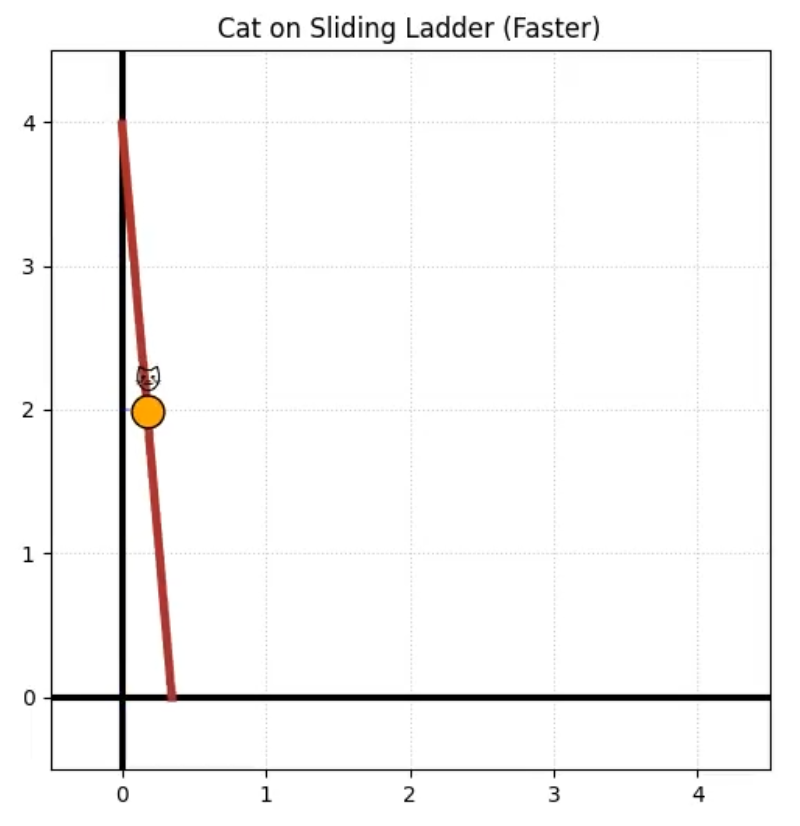
\includegraphics[width=\linewidth]{image_1.png} 
        \caption{Frame 1: Ladder starts sliding.}
    \end{subfigure}
    \hfill
    % Box 2 (Top Right)
    \begin{subfigure}[b]{0.45\textwidth}
        \centering
        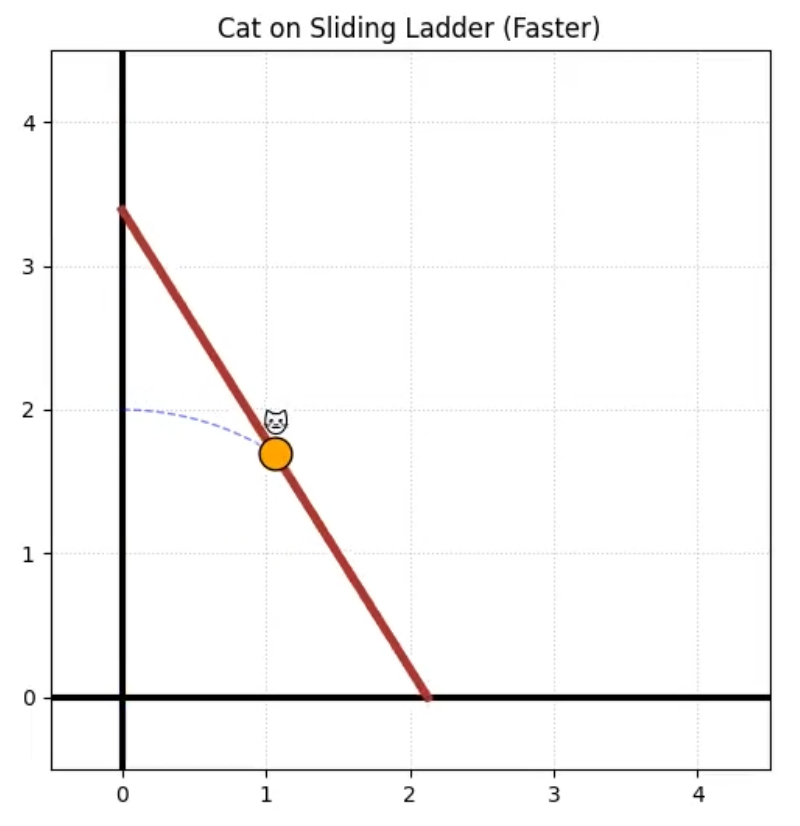
\includegraphics[width=\linewidth]{image_2.png}
        \caption{Frame 2: Cat's path begins.}
    \end{subfigure}
    
    \vspace{0.5cm} % Space between rows
    
    % Box 3 (Bottom Left)
    \begin{subfigure}[b]{0.45\textwidth}
        \centering
        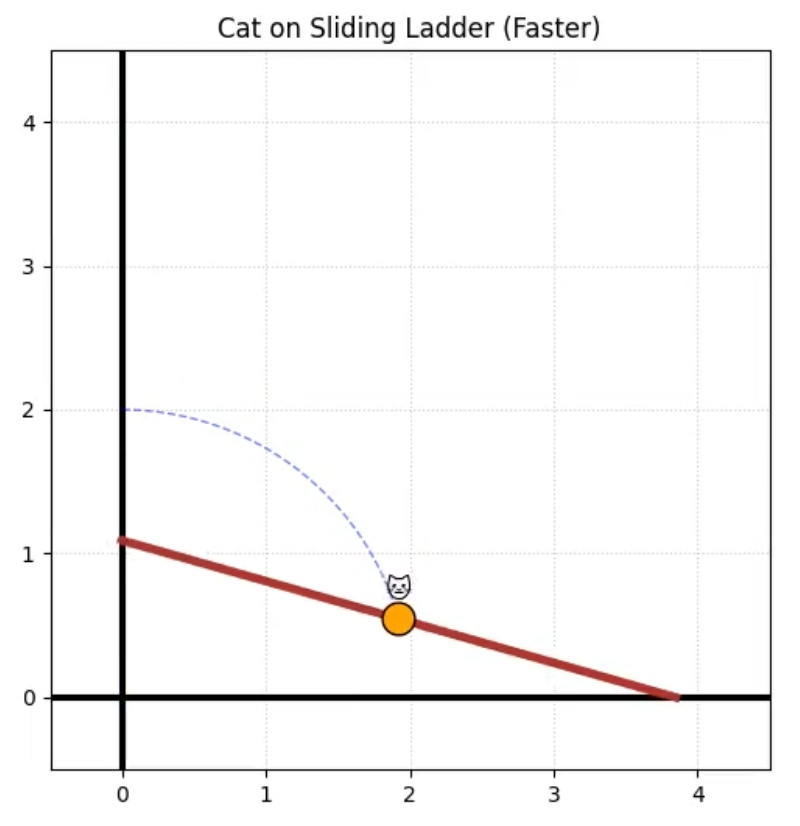
\includegraphics[width=\linewidth]{image_3.png}
        \caption{Frame 3: Circular arc becomes visible.}
    \end{subfigure}
    \hfill
    % Box 4 (Bottom Right)
    \begin{subfigure}[b]{0.45\textwidth}
        \centering
        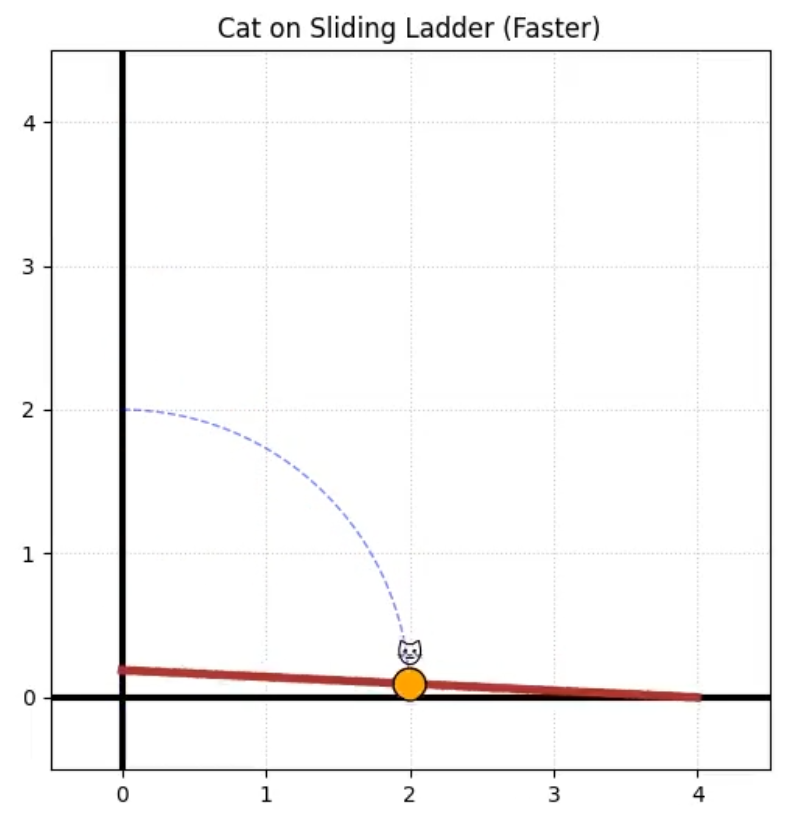
\includegraphics[width=\linewidth]{image_4.png}
        \caption{Frame 4: Ladder hits the floor.}
    \end{subfigure}
    
    \caption{The Cat on the Sliding Ladder: A visual progression over time.}
    \label{fig:sliding_ladder_grid}
\end{figure}
\vspace{1cm}

% ======================================================================
% GITHUB REPOSITORY LINK BOX 
% ======================================================================
\begin{mdframed}[backgroundcolor=gray!10, linecolor=black, linewidth=1pt, roundcorner=5pt]
    \centering
    \textbf{Interactive Code Available!} \\
    \vspace{0.2cm}
    You can view, run, and experiment with the full Python source code for the sliding ladder animation and other geometries in the official GitHub repository: \\
    \vspace{0.3cm}
    
    \small 
    \href{https://github.com/Shubham18024/Python-Mathematical-Animation/blob/main/2d-anim/scripts/cat_at_middle_ladder.py}{
        \color{blue}\underline{Click here to view: cat\_at\_middle\_ladder.py}
    } \\
    \vspace{0.1cm}
    \scriptsize \texttt{https://github.com/Shubham18024/Python-Mathematical-Animation/} \\
    \texttt{blob/main/2d-anim/scripts/cat\_at\_middle\_ladder.py}
\end{mdframed}
% ======================================================================


\section{The Concept of Equivalent Norms}

In our journey from basic geometry to advanced mathematics, we encounter the concept of a \textbf{norm}. A norm is essentially a mathematical ruler used to measure the "size" or "length" of a vector in a space $X$. However, just as you can measure a table in inches or centimeters, mathematicians can measure vector spaces using different norms.

A critical question arises: Do different norms change the fundamental nature of the space? For finite-dimensional spaces like $\mathbb{R}^2$, the answer is a comforting "No". We call these \textbf{Equivalent Norms}. According to Kreyszig \cite{kreyszig1989} (Definition 2.4-4), two norms $||\cdot||$ and $||\cdot||_0$ are equivalent if they satisfy the following inequality for some positive constants $a$ and $b$:
\begin{equation}
    a||x||_{0} \le ||x|| \le b||x||_{0}
\end{equation}
This ensures that if a vector is considered "small" by one norm, it is also "small" by the other \cite{kreyszig1989}. While the specific "shape" of the distance might change, the underlying topology—the open sets and convergent sequences—remains identical.

\section{The $l_p$ Unit Ball: From Diamonds to Squares}

To visualize this, we look at the $l_p$ unit ball, defined by the set of points $(x, y)$ such that:
\begin{equation}
    |x|^p + |y|^p = 1
\end{equation}
As we vary the value of $p$, the geometry of the "unit circle" undergoes a fascinating transformation:
\begin{itemize}
    \item \textbf{$p=1$}: The unit ball is a diamond (the Manhattan norm).
    \item \textbf{$p=2$}: The unit ball is the familiar Euclidean circle.
    \item \textbf{$p \to \infty$}: The unit ball expands into a square (the Supremum norm).
\end{itemize}

Our animation will show a single point moving around these boundaries, demonstrating how the "usual circle" is continuously warped into different $l_p$ shapes while maintaining the same topological properties.

\section{The Parametrization Strategy}

To animate this transition smoothly, we cannot use the standard $x^2 + y^2 = 1$ logic. We need a general parametrization that works for any value of $p$. We use the following transformation based on the sign function (\textit{sgn}) to ensure we cover all four quadrants:
\begin{align}
    x(t) &= \text{sgn}(\cos t) |\cos t|^{2/p} \\
    y(t) &= \text{sgn}(\sin t) |\sin t|^{2/p}
\end{align}
This ensures that $|x(t)|^p + |y(t)|^p = |\cos t|^2 + |\sin t|^2 = 1$, perfectly placing every point on the boundary for any $p$.

\section{Implementation: The Norm Animation Engine}

The following Python code \cite{python_docs} implements this warping geometry. It uses a dual-loop logic: one loop to change the value of $p$ and another to trace the boundary dynamically via Matplotlib \cite{matplotlib_docs}.

\begin{lstlisting}[caption={Animating Equivalent Norms in $\mathbb{R}^2$}]
import numpy as np
import matplotlib.pyplot as plt
import matplotlib.animation as animation

# Define the p-values we want to visualize
p_values = [1, 2, 3, 5, 10, 20, np.inf]
points_per_norm = 200

def lp_unit_ball(p, num_points=200):
    t = np.linspace(0, 2*np.pi, num_points)
    if p == np.inf:
        # Special case for the square (L-infinity)
        x = np.array([1]*50 + list(np.linspace(1,-1,50)) + [-1]*50 + list(np.linspace(-1,1,50)))
        y = np.array(list(np.linspace(-1,1,50)) + [1]*50 + list(np.linspace(1,-1,50)) + [-1]*50)
        return x, y
    
    # General p-norm parametrization
    x = np.sign(np.cos(t)) * np.abs(np.cos(t))**(2/p)
    y = np.sign(np.sin(t)) * np.abs(np.sin(t))**(2/p)
    return x, y

fig, ax = plt.subplots(figsize=(6,6))
line, = ax.plot([], [], 'r-', lw=2)
point, = ax.plot([], [], 'bo')

def update(frame):
    # Determine which p-value and which point on the curve we are at
    p_idx = (frame // points_per_norm) % len(p_values)
    t_idx = frame % points_per_norm
    
    p = p_values[p_idx]
    x_full, y_full = lp_unit_ball(p)
    
    line.set_data(x_full, y_full)
    point.set_data([x_full[t_idx]], [y_full[t_idx]])
    ax.set_title(f"L_p Unit Ball (p = {p})")
    return line, point

ani = animation.FuncAnimation(fig, update, frames=len(p_values)*points_per_norm, interval=20)
plt.show()
\end{lstlisting}

\subsection{Understanding the Code Logic}
\begin{itemize}
    \item \textbf{The \texttt{lp\_unit\_ball} Function:} This converts our mathematical parametrization into NumPy arrays. For the $L_\infty$ norm, we handle it as a special case to ensure the square edges are perfectly sharp.
    \item \textbf{The Frame Management:} In the \texttt{update} function, we use the floor division (\texttt{//}) and modulo (\texttt{\%}) operators. This allows us to cycle through multiple $p$ values in a single continuous animation run.
    \item \textbf{Dynamic Titles:} We use f-strings (\texttt{f"L\_p Unit Ball (p = \{p\})" }) to update the title in real-time, helping the viewer track which norm is currently being displayed.
\end{itemize}

% ======================================================================
% 4-PHOTO GRID FOR THE L_p UNIT BALLS
% ======================================================================
\begin{figure}[h!]
    \centering
    \begin{subfigure}[b]{0.45\textwidth}
        \centering
        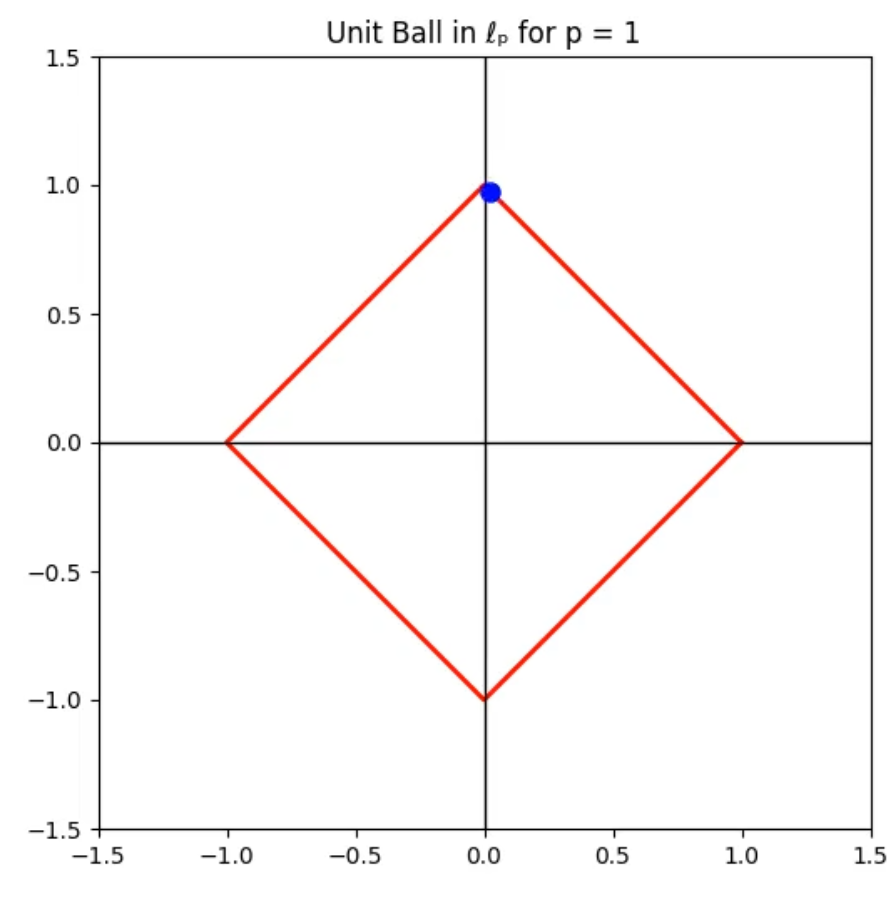
\includegraphics[width=\linewidth]{norm_p1.png} 
        \caption{$p=1$: The Diamond Shape.}
    \end{subfigure}
    \hfill
    \begin{subfigure}[b]{0.45\textwidth}
        \centering
        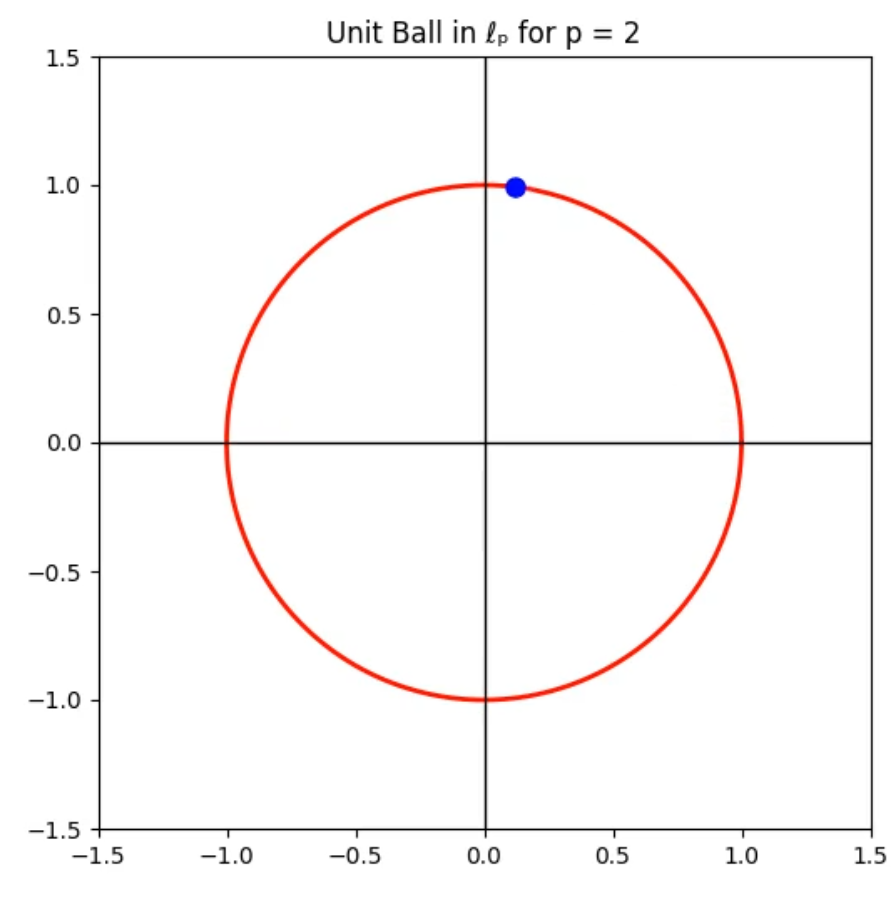
\includegraphics[width=\linewidth]{norm_p2.png}
        \caption{$p=2$: The Standard Circle.}
    \end{subfigure}
    
    \vspace{0.5cm} 
    
    \begin{subfigure}[b]{0.45\textwidth}
        \centering
        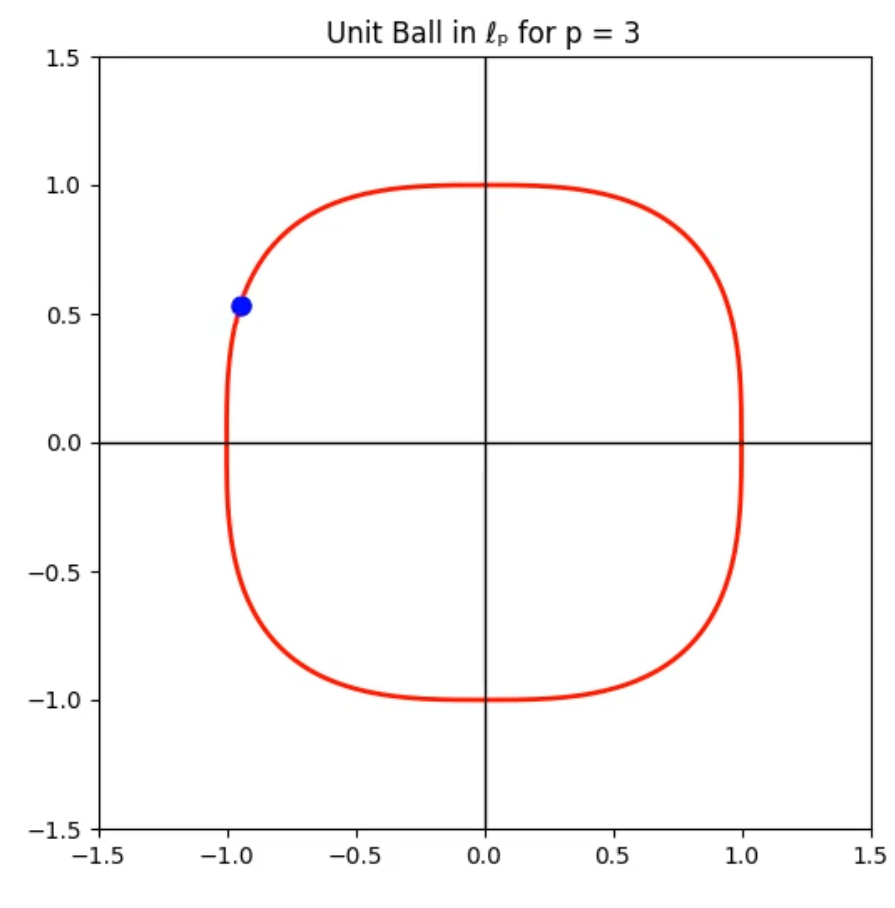
\includegraphics[width=\linewidth]{norm_p3.png}
        \caption{$p=3$: Warping towards a square.}
    \end{subfigure}
    \hfill
    \begin{subfigure}[b]{0.45\textwidth}
        \centering
        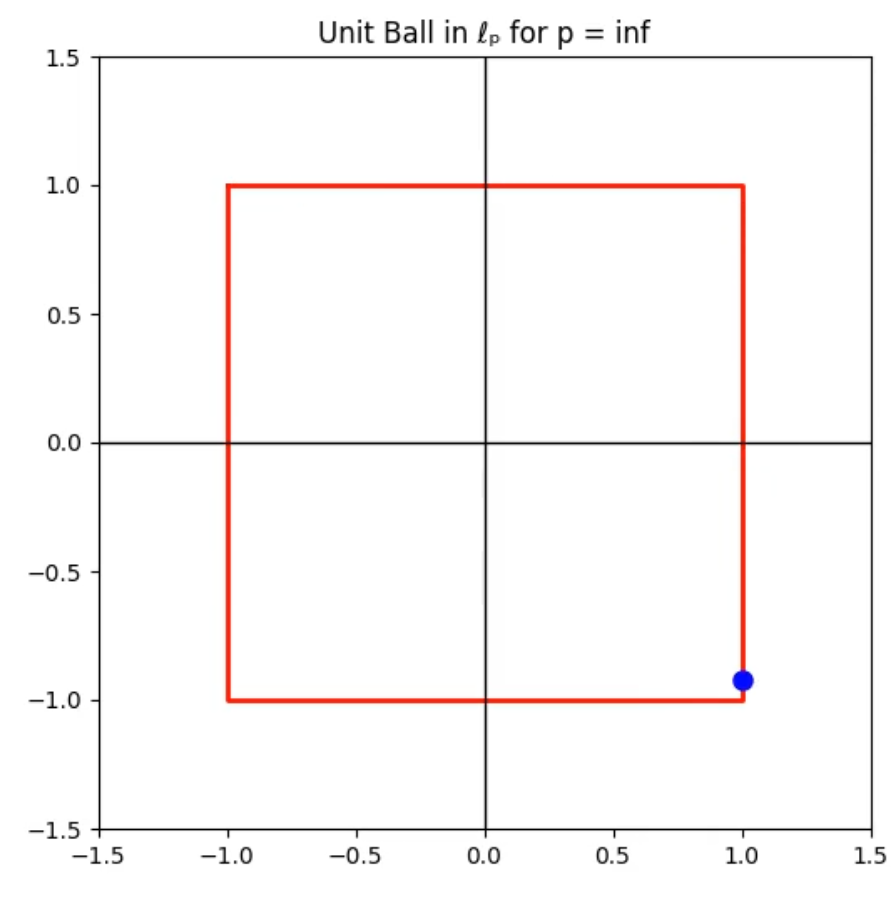
\includegraphics[width=\linewidth]{norm_pinf.png}
        \caption{$p=\infty$: The Square Boundary.}
    \end{subfigure}
    
    \caption{Visual progression of the $l_p$ unit ball as $p$ increases.}
    \label{fig:lp_norms_grid}
\end{figure}

%================================================================
%================================================================
% ... (This continues immediately after \label{fig:lp_norms_grid} \end{figure}) ...

\newpage
\section{Plotting Implicit Functions: The Ellipse}

After understanding basic circles, we extend our animation engine to the ellipse. The general implicit equation of an ellipse centered at $(h, k)$ with a semi-major axis $a$ and semi-minor axis $b$ is:
\begin{equation}
    \frac{(x-h)^2}{a^2} + \frac{(y-k)^2}{b^2} = 1
\end{equation}

\vspace{0.5cm}
\noindent
\begin{minipage}{0.6\textwidth}
    Just as we saw with earlier geometries \cite{loney1895}, plotting directly from the implicit form is difficult for computers because it requires computing multiple $y$-values for a single $x$-value, leading to broken lines and rendering issues. 
    
    Therefore, we parametrize the ellipse using an angle parameter $t$. This traces the ellipse smoothly using sine and cosine functions:
    \begin{align}
        x(t) &= h + a\cos(t) \\
        y(t) &= k + b\sin(t)
    \end{align}
    
    In the code implementation below, we use Python \cite{python_docs} and Matplotlib \cite{matplotlib_docs} to animate a single point traveling along this path. The main logic involves computing the parametric coordinates for each frame and updating the position of our point object continuously.
\end{minipage}
\hfill
\begin{minipage}{0.35\textwidth}
    \centering
    % Replace 'example-image' with your actual ellipse image filename
    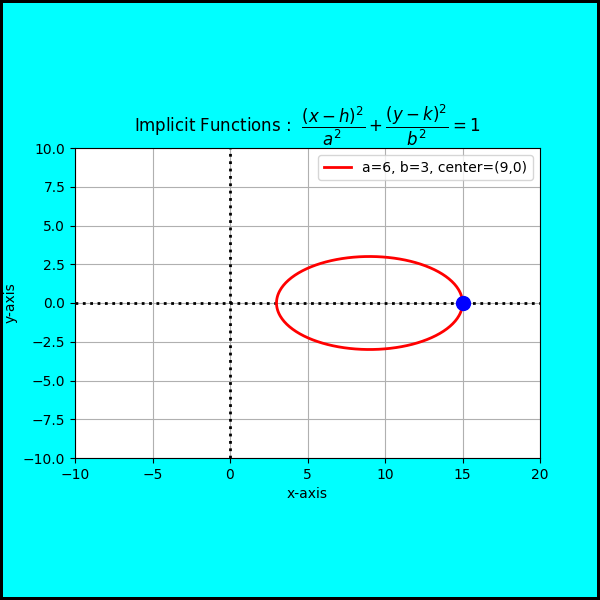
\includegraphics[width=\linewidth]{ellipse.png} 
    \vspace{0.2cm}
    
    \small \textit{Fig: Parametric path of an ellipse.}
\end{minipage}
\vspace{0.5cm}

% --- Parametrization Box & Author Tip ---
\noindent
\begin{minipage}[t]{0.65\textwidth}
    \vspace{0pt}
    \begin{mdframed}[backgroundcolor=gray!10, linecolor=black, linewidth=1pt, roundcorner=5pt]
        \textbf{Parametrization of General Shapes} \\
        \vspace{0.2cm}
        \small
        \begin{itemize}
            \item \textbf{Line Segment} (from $(x_1, y_1)$ to $(x_2, y_2)$): \\
            $x(t) = x_1 + t(x_2 - x_1)$ \\
            $y(t) = y_1 + t(y_2 - y_1)$ \quad for $t \in [0, 1]$
            
            \vspace{0.1cm}
            \item \textbf{Parabola} ($y^2 = 4ax$): \\
            $x(t) = at^2$ \\
            $y(t) = 2at$ \quad for $t \in (-\infty, \infty)$
            
            \vspace{0.1cm}
            \item \textbf{Hyperbola} ($\frac{x^2}{a^2} - \frac{y^2}{b^2} = 1$): \\
            $x(t) = a \sec(t)$ \\
            $y(t) = b \tan(t)$ \quad for $t \in [0, 2\pi)$
        \end{itemize}
    \end{mdframed}
\end{minipage}
\hfill
\begin{minipage}[t]{0.3\textwidth}
    \vspace{0pt}
    \scriptsize \textbf{Author Tip:}\\
    The transition from implicit to parametric forms is a universal strategy in computational geometry. For any general shape defined by $f(x, y) = 0$, finding a set of equations $x = g(t)$ and $y = h(t)$ allows us to map a single 1D time array $t$ directly to 2D space. This avoids vertical line test failures and infinite slopes, making it the most robust mathematical approach for programmatic drawing and animation.
\end{minipage}
\vspace{0.5cm}

\begin{lstlisting}[caption={Animating a Point on an Ellipse}]
import numpy as np
import matplotlib.pyplot as plt
import matplotlib.animation as animation

def setup_axes():
    fig, ax = plt.subplots(figsize=(6,6), dpi=100)
    ax.set_xlim(-10, 20)
    ax.set_ylim(-10, 10)
    ax.axhline(0, color="black", linewidth=2, linestyle=":")
    ax.axvline(0, color="black", linewidth=2, linestyle=":")
    ax.set_aspect("equal", adjustable="box")
    ax.grid(True)
    ax.set_title("Implicit Functions : Ellipse")
    return fig, ax

def starting_position():
    point.set_data([], [])
    return point,

def update_frame(frame, a, b, h, k):
    # Main logic: Update point position using parametric equations
    point.set_data([h + a*np.cos(frame)], [k + b*np.sin(frame)])
    return point,

# Ellipse parameters
a, b = 6, 3
h, k = 9, 0

set_of_points = np.linspace(0, 2*np.pi, 300)
figure, ax = setup_axes()

# Plot the static path
ax.plot(h + a*np.cos(set_of_points), k + b*np.sin(set_of_points), 
        linewidth=2, color="red")
point, = ax.plot([], [], "bo", markersize=10)

ani = animation.FuncAnimation(
    fig=figure, func=update_frame, frames=set_of_points,
    fargs=(a,b,h,k), init_func=starting_position,
    interval=30, blit=True)

plt.show()
\end{lstlisting}

\newpage
\section{Stochastic Geometry: The 2D Random Walk}

\noindent
\begin{minipage}{0.6\textwidth}
    Moving beyond deterministic geometric shapes, mathematical animation can also visualize probabilistic systems. A 2D random walk models a path consisting of a succession of random steps on a mathematical space. 

    The main logic in the Python \cite{python_docs} script relies on generating a random integer between 1 and 4 for every frame. Depending on the result, the current $X$ or $Y$ coordinate is incremented or decremented by 1. These new coordinates are appended to an array, and Matplotlib \cite{matplotlib_docs} continuously redraws the line to show the growing, randomized trail over time.
\end{minipage}
\hfill
\begin{minipage}{0.35\textwidth}
    \centering
    % Replace 'example-image' with your actual random walk image filename
    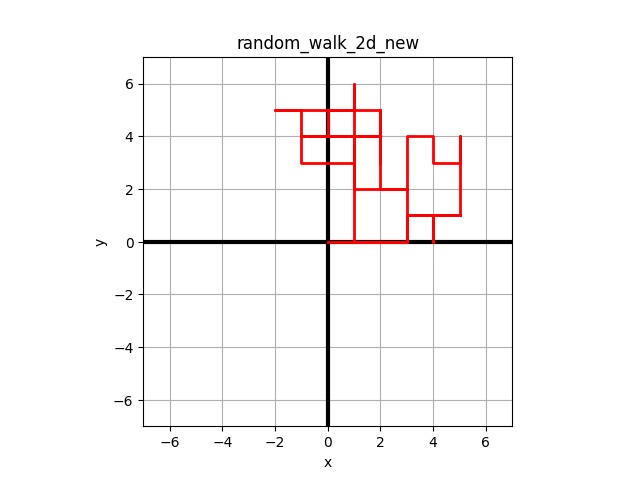
\includegraphics[width=\linewidth]{random_walk.png} 
    \vspace{0.2cm}
    
    \small \textit{Fig: 2D Random Walk Path.}
\end{minipage}
\vspace{0.5cm}

\begin{lstlisting}[caption={Simulating a 2D Random Walk}]
import numpy as np
import matplotlib.pyplot as plt
import matplotlib.animation as animation

fig, axs = plt.subplots()
axs.set_xlim(-7, 7)
axs.set_ylim(-7, 7)
axs.axhline(0, color='black', linewidth=3)   
axs.axvline(0, color='black', linewidth=3) 
axs.set_aspect('equal', adjustable='box')

x, y = [0], [0]
path_line, = axs.plot([], [], 'r-', linewidth=2)

def init():
    x.clear()
    y.clear()
    x.append(0)
    y.append(0)
    path_line.set_data([], [])
    return path_line,

def update(frame):
    xold = x[-1]
    yold = y[-1]
    
    # Main logic: Pick a random direction (1: Right, 2: Left, 3: Up, 4: Down)
    rnd = np.random.randint(1, 5)
    if rnd == 1:
        xnew, ynew = xold + 1, yold
    elif rnd == 2:
        xnew, ynew = xold - 1, yold
    elif rnd == 3:
        xnew, ynew = xold, yold + 1
    else:
        xnew, ynew = xold, yold - 1
        
    x.append(xnew)
    y.append(ynew)
    path_line.set_data(x, y)
    return path_line,

ani = animation.FuncAnimation(fig, update, frames=100, 
                              init_func=init, blit=True, interval=50)
plt.title("2D Random Walk")
plt.grid(True)
plt.show()
\end{lstlisting}

\newpage
\section{Dynamic Transformations: Rotating a Curve}

\noindent
\begin{minipage}{0.6\textwidth}
    Mathematical animation is uniquely suited to display linear transformations, such as rotations, as a continuous motion rather than a simple "before and after" state. In this example, we apply a rotation matrix to a standard sine curve.

    The core logic requires defining our base curve coordinates ($x_c$ and $y_c$). For each frame, we treat the frame parameter $k$ as our rotation angle $\theta$. We then apply the standard 2D rotation matrix \cite{loney1895} to every point on the curve simultaneously:
    \begin{align}
        x &= x_c \cos(k) - y_c \sin(k) \\
        y &= x_c \sin(k) + y_c \cos(k)
    \end{align}
    By feeding these updated arrays into Matplotlib \cite{matplotlib_docs}, the entire curve appears to spin smoothly around the origin.
\end{minipage}
\hfill
\begin{minipage}{0.35\textwidth}
    \centering
    % Replace 'example-image' with your actual rotating curve image filename
    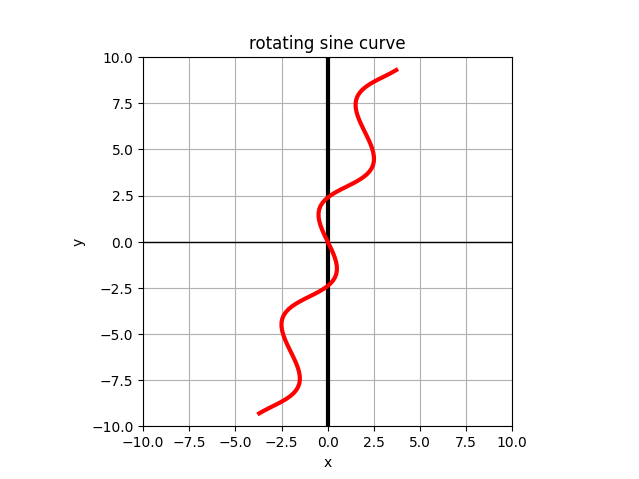
\includegraphics[width=\linewidth]{sine_curve.png} 
    \vspace{0.2cm}
    
    \small \textit{Fig: Rotating Sine Curve.}
\end{minipage}
\vspace{0.5cm}

\begin{lstlisting}[caption={Animating a Rotating Sine Curve}]
import numpy as np
import matplotlib.pyplot as plt
import matplotlib.animation as animation

fig, axs = plt.subplots()
axs.set_xlim(-10, 10)
axs.set_ylim(-10, 10)
axs.axhline(0, color='black', linewidth=1)   
axs.axvline(0, color='black', linewidth=1) 
axs.set_aspect('equal', adjustable='box')

# Time frames act as our rotation angle
t = np.linspace(-np.pi/2 + 0.01, np.pi/2 - 0.01, 100)
# Base coordinates for the sine curve
u = np.linspace(-10, 10, 100)

straight_line, = axs.plot([], [], linestyle='-', color='red', linewidth=3)

def init():
    straight_line.set_data([], [])
    return straight_line,   

def update(frame):
    k = frame # Current rotation angle
    xc = u
    yc = np.sin(u)
    
    # Main logic: Apply 2D rotation matrix to the coordinates
    x = xc*np.cos(k) - yc*np.sin(k)
    y = xc*np.sin(k) + yc*np.cos(k)
    
    straight_line.set_data(x, y)
    return straight_line,   

ani = animation.FuncAnimation(fig, update, frames=t, 
                              init_func=init, blit=True, interval=50)

axs.set_title("Rotating Sine Curve")
axs.grid(True)
plt.show()
\end{lstlisting}

% ===============================================================
% ===============================================================
\newpage
\section{Further Explorations and Open Source Contributions in 2d}

The animations detailed in this chapter—from the sliding ladder and equivalent norms to parametric ellipses and random walks—represent only a fraction of what is possible using this computational approach. 

The complete suite of two-dimensional mathematical animations is actively maintained in a dedicated open-source repository. Beyond the scripts discussed, the repository contains several other foundational animations, including:
\begin{itemize}
    \item \textbf{\texttt{amplitude\_of\_sine\_wave.py}:} Visualizing how changing the amplitude coefficient dynamically stretches and compresses a waveform.
    \item \textbf{\texttt{unit\_circle\_anim.py}:} The foundational script demonstrating the parametric generation of a standard circle using sine and cosine over time.
\end{itemize}

\vspace{0.5cm}
% --- GitHub Contribution Box ---
\begin{mdframed}[backgroundcolor=gray!10, linecolor=black, linewidth=1pt, roundcorner=5pt]
    \centering
    \textbf{Explore the Repository \& Contribute!} \\
    \vspace{0.3cm}
    \raggedright
    All 2D scripts are publicly available in the \texttt{2d-anim} directory of the official project repository. You are encouraged to view, run, and modify these files to build your own mathematical intuition.
    
    \vspace{0.3cm}
    \centering
    \href{https://github.com/Shubham18024/Python-Mathematical-Animation/tree/main/2d-anim}{
        \color{blue}\underline{View the 2D Animations Folder on GitHub}
    } \\
    \vspace{0.1cm}
    \scriptsize \texttt{https://github.com/Shubham18024/Python-Mathematical-Animation/tree/main/2d-anim}
    
    \vspace{0.4cm}
    \raggedright
    \textbf{Call for Contributions:} \\
    Mathematics is a collaborative discipline. If you have an idea for a new geometric visualization, a physics simulation, or an improvement to an existing script, you are welcome to fork the repository, write your animation, and submit a Pull Request!
\end{mdframed}
\vspace{0.5cm}
%================================================================
\newpage
\newpage
\section{Project Environment and Dependency Management using UV}

To ensure complete reproducibility and efficient dependency management across different machines, this entire project is managed using \textbf{uv} \cite{uv_docs}. Developed by Astral, \texttt{uv} is an extremely fast Python package and project manager written in Rust. It is designed as a modern, high-performance drop-in replacement for standard tools like \texttt{pip}, \texttt{virtualenv}, and \texttt{pip-tools}.

When dealing with mathematical animations, version control of libraries is critical. A slight update in how \texttt{Matplotlib} handles rendering backends or how \texttt{NumPy} processes specific array broadcasting can break an animation script that previously worked perfectly. By utilizing \texttt{uv}, we maintain a strict \texttt{pyproject.toml} and \texttt{uv.lock} file. This guarantees that anyone who clones this repository will build the exact same isolated virtual environment, instantly, without dealing with version conflicts or broken dependencies.

\subsection{Workflow 1: Cloning and Running the Existing Project}
For educators, evaluators, or students who simply want to view the animations locally, \texttt{uv} makes the setup process virtually instantaneous. You do not need to manually create virtual environments or guess which library versions to install.

\vspace{0.2cm}
\begin{mdframed}[backgroundcolor=gray!10, linecolor=black, linewidth=1pt, roundcorner=5pt]
    \textbf{Terminal Commands to Run the Project:}
    \vspace{0.1cm}
    \begin{verbatim}
# 1. Clone the official GitHub repository
git clone https://github.com/Shubham18024/Python-Mathematical-Animation.git
cd Python-Mathematical-Animation

# 2. Sync the project (uv creates a virtual environment and 
# installs the exact dependencies from uv.lock instantly)
uv sync

# 3. Run any animation script safely inside the isolated environment
uv run 2d-anim/scripts/cat_at_middle_ladder.py
    \end{verbatim}
\end{mdframed}
\vspace{0.4cm}

\subsection{Workflow 2: Starting a New Animation Project from Scratch}
If you are inspired to create your own repository of mathematical animations, \texttt{uv} simplifies the initialization phase \cite{uv_docs}. Instead of juggling \texttt{python -m venv venv} and \texttt{pip install}, you can scaffold a robust project in seconds.

\vspace{0.2cm}
\begin{mdframed}[backgroundcolor=gray!10, linecolor=black, linewidth=1pt, roundcorner=5pt]
    \textbf{Terminal Commands for New Contributors:}
    \vspace{0.1cm}
    \begin{verbatim}
# 1. Initialize a new Python project (creates pyproject.toml)
uv init my_math_animations
cd my_math_animations

# 2. Add the core mathematical and plotting libraries
# This automatically updates pyproject.toml and installs them
uv add numpy matplotlib

# 3. Execute your new script without activating environments
uv run main.py
    \end{verbatim}
\end{mdframed}
\vspace{0.3cm}

The use of \texttt{uv} in this project not only demonstrates modern software engineering practices but also ensures that the focus remains entirely on the mathematics and logic, rather than wasting time debugging Python environments.

\newpage
\section{Expanding into the Third Dimension}
While this current work focuses heavily on two-dimensional parametrizations and animations, the true power of this computational approach is unleashed when we move into 3D space. In our future work, we plan to extend this visualization framework towards fully three-dimensional problems. By utilizing $X$, $Y$, and $Z$ coordinate transformations, we can animate complex surfaces like the Torus, Catenoid, and Helicoid. This will involve applying rotation matrices and translating coordinate points to manipulate 3D shapes programmatically, offering a profound way to teach multivariable calculus and spatial geometry.


\section{Official Code Repository}
All the core foundations, current 2D scripts, and upcoming 3D algorithms are actively maintained and available for experimentation. Students, educators, and developers can access the complete source code, track the project's evolution, and view the future 3D implementations at the official GitHub repository:

\vspace{0.4cm}
\begin{mdframed}[backgroundcolor=gray!10, linecolor=black, linewidth=1pt, roundcorner=5pt]
    \centering
    \textbf{Project GitHub Repository:} \\
    \vspace{0.2cm}
    \href{https://github.com/Shubham18024/Python-Mathematical-Animation}{\texttt{https://github.com/Shubham18024/Python-Mathematical-Animation}}
\end{mdframed}
\vspace{0.5cm}

% --- Bibliography ---
% --- Bibliography ---
\begin{thebibliography}{9}

\bibitem{python_docs}
Python Software Foundation. (2026). \textit{Python Language Reference}. Retrieved from \url{https://docs.python.org/3/}

\bibitem{matplotlib_docs}
Matplotlib Developers. (2026). \textit{Matplotlib Animation Guide}. Retrieved from \url{https://matplotlib.org/}

\bibitem{loney1895}
Loney, S. L. (1895). \textit{The Elements of Coordinate Geometry}. London: Macmillan and Co.

\bibitem{kreyszig1989}
Kreyszig, Erwin (1989). \textit{Introductory Functional Analysis with Applications} (1st ed.). John Wiley \& Sons. Wiley-India Student Edition. Indian Reprint 2007.

\bibitem{uv_docs}
Astral. (2024). \textit{uv: First steps}. Retrieved from \url{https://docs.astral.sh/uv/getting-started/first-steps/}

\end{thebibliography}

\end{document}